% Author attachment: pasted-text-2026-10-10_23-16-35-189.md

% Wording and values preserved; only LaTeX escaping and reference integration.

\section{Ablations}

% Queue Figure 5 early so it can occupy the top-left column on page 7.
\begingroup
\let\ablationfigure\figure
\renewcommand{\figure}[1][]{\ablationfigure[!t]}
\begin{figure}[!htbp]
\centering
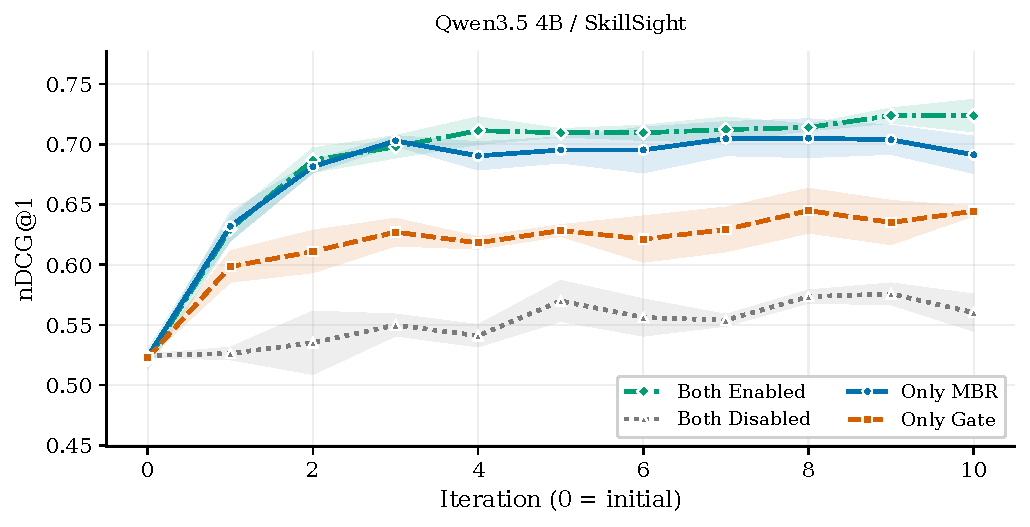
\includegraphics[width=\linewidth]{figs/mbr_replay_test_ndcg@1_std/preview.pdf}
\caption[Replay and validation-gate ablation: test nDCG@1]{\input{figs/mbr_replay_test_ndcg@1_std/description.text}}
\label{fig:mbr_replay_test_ndcg@1_std}
\end{figure}

\endgroup

\subsection{Impact of MBR based on Replay and Held-out Validation Gate}

Figure~\ref{fig:mbr_replay_test_ndcg@1_std} shows test nDCG@1 across three runs per configuration with SkillSight; the following F1 and nDCG@10 results provide complementary metrics. MBR with bounded replay alone achieved higher final performance on test dataset than the held-out validation gate alone: F1 increased from 0.495 to 0.594 and nDCG@10 from 0.722 to 0.776, relative improvements of 20.0\% and 7.4\%, respectively. Combining MBR with the held-out gate further improved final performance on unseen test tasks, increasing F1 by 3.28\% and nDCG@10 by 1.21\% compared with MBR alone. Relative to each configuration's own initialization, disabling both only increases F1 and nDCG@10 by 21.0\% and 8.3\% which is much lower than the 100.9\% and 24.1\% increase when both are enabled. This supports empirical update selection without implying that unchecked updates invariably worsen performance. With both components enabled, diminishing returns appeared around iteration 5, by which point 96.5\% of the final F1 gain and 95.7\% of the final nDCG@10 gain had accrued. Later iterations added only 0.011 F1 and 0.007 nDCG@10, indicating an approximate plateau. This suggest diminishing opportunities for useful predicate refinement on the plateau: early iterations correct broad, frequent routing errors, while later iterations encounter harder or less common cases.

\subsection{Performance and Token Usage Tradeoff of MBR Replay and Held-out Gate}

Figure~\ref{fig:performance_token_usage} shows that combining replay and the gate provides the strongest final routing performance, while MBR alone reduces token usage by 10.8\% at the cost of a 7.7\% relative decrease in nDCG@1 compared with Both Enabled. Across configurations with and without the gate, enabling replay improves final routing performance by 15.4\% to 23.7\%, while increasing known run-local token usage by 40.6\% to 52.9\%.

\subsection{Skill Routing Performance across LLM Backbones}

The results show that cold-start performance of RouterBSI’s predicates created from skills without task feedback increases as the LLM backbone becomes more capable. For instance, the cold-start nDCG@1 of Qwen 3.5 4B is 0.520 whereas Qwen 3.8 27B and GPT-OSS 120B performance is 0.635 and 0.686 (Figure~\ref{fig:routing_performance_across_llms_init}). The routing performance gains from RouterBSI optimization range from 42.7\% to 8.6\% decreasing with model size. The decrease in performance gained is likely cause by a plateau in routing performance between 0.742 and 0.802. Another notable result is that RouterBSI improved performance of the smaller Qwen3.5 4B enough to reach the performance of GPT-OSS,  a model with over 115b more parameters.

\begin{figure}[!htbp]
\centering
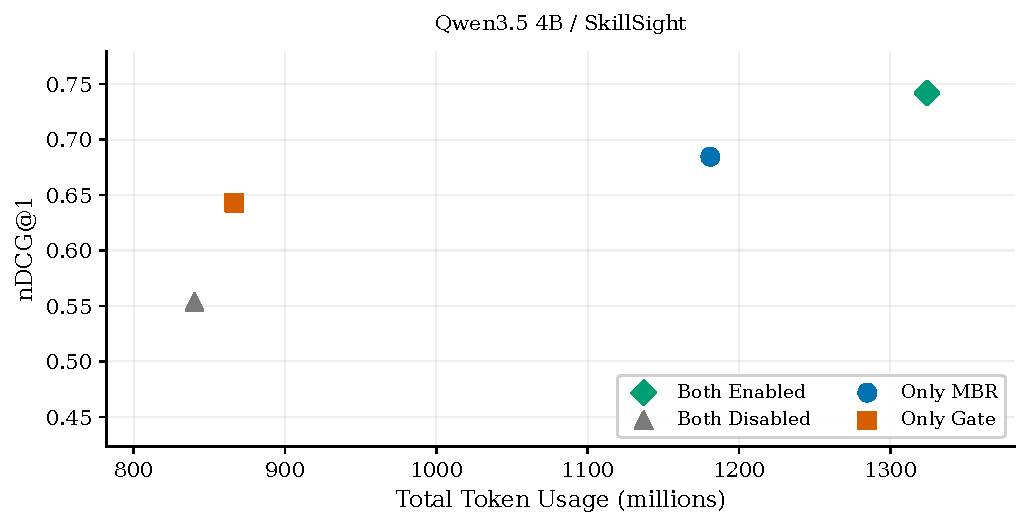
\includegraphics[width=\linewidth]{figs/performance_token_usage/preview.pdf}
\caption{Routing performance and optimization token usage with replay and validation gating enabled or disabled. Points show task-weighted test nDCG@10 against recorded run-local tokens in millions. These exploratory results use incomplete token totals that exclude shared initialization.}
\label{fig:performance_token_usage}
\end{figure}


% Defer Figure 7 after Figure 6 is numbered, while prose continues to flow.
\afterpage{%
\begingroup
\let\backbonepagefigure\figure
\renewcommand{\figure}[1][]{\backbonepagefigure[!ht]}
\begin{figure}[!htbp]
\centering
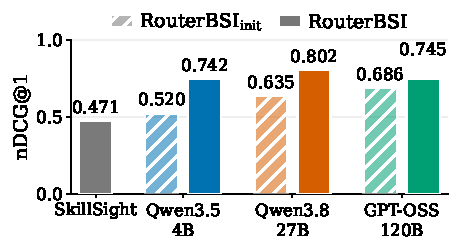
\includegraphics[width=\linewidth]{figs/routing_performance_across_llms_init/preview.pdf}
\caption[Routing performance by language-model backbone]{\input{figs/routing_performance_across_llms_init/description.text}}
\label{fig:routing_performance_across_llms_init}
\end{figure}

\endgroup
}

